\documentclass{article}

\usepackage[margin=1.5cm]{geometry}
\usepackage{titlesec}
% \usepackage{amsmath}
\usepackage{mathtools}
\usepackage{amsthm}
\usepackage{xcolor}
\usepackage{soul}
\usepackage{multicol}
\usepackage{multirow}
\usepackage{amsfonts}
\usepackage{setspace}
\usepackage{graphicx}
\usepackage{hyperref}
\usepackage{listings}

% SETUP
% \geometry{letterpaper}
\onehalfspacing

\graphicspath{ {./imgs/} }

\title{PV251: Visualization; Semestral Project --- Report}
\author{Jakub Čillík}
\date{\today}

% \titleformat*{\subsection}{\fontsize{14}{20}\selectfont\bfseries}
% \titleformat*{\subsubsection}{\fontsize{12}{20}\selectfont\bfseries}

% \titlespacing*{\subsection}{0pt}{*1}{3pt}
% \titlespacing*{\subsubsection}{0pt}{*1}{2pt}

\makeatletter
\newcommand{\hlm}[2][yellow]{\colorbox{#1}{$\displaystyle #2$}}

\begin{document}
    \noindent
    \textbf{PV251: Visualization}\hfill\textbf{Semestral Project --- Report}\\
    \@author, UČO: \textbf{524749}
    \vspace{0.5em}
    \hrule

    \vspace{1.5em}
    \noindent
    {\huge \textbf{Visualizing personal spending data}}

    \subsection*{Motivation}
        The core idea induced in the past, when I started to track my personal expenses. Without deeper knowledge about charts and visuliazations, I created a simple project to record, preprocess and plot the gathered data in a primitive way. The main goal of this project is to visualize the data in a more sophisticated way, using more advanced visualization techniques and tools.

        \subsubsection*{Description}
            The layout consist of several charts, each representing a different aspect of the data. Starting with a line chart showing the monthly sum over entire period when the data was recorded. The second chart shows comparison between last 12 months and previous 12 months.
            The next section is dedicated to filters. Available options are to select particular categories and/or to select a time range. The next two charts are mass chart and cumulative distribution over month. Another chart is violin plot presenting analysis for each category, followed by a barplot showing the number of records for each category during selecter time range. Lastly a treemap is used to visualize how much money was spent in each category.
    
    \subsection*{Dataset}
        The dataset is a collection of personal expenses, recorded in a CSV file. Considering the publicness of the project, the exact data is sampled and randomized from the original dataset.

        \subsubsection*{Preprocessing}
            Preprocessing consists of calculating the stats for particular charts. The data is filtered based on the selected time range and categories. The data is then grouped by month and category, and the stats are calculated. The data is then used to plot the charts.\\[1em]
            Fields are exactly as defined in the database.
    
    \subsection*{Used Technology}
        The project is web-based, coded in TypeScript using React library. For data manipulation, data-forge library is used. For visualizations, Chartj.js libary is used. Additionally, the application is fully containerized using Docker.

    \subsection*{Running the Project}
        Project is deployed at \url{https://cillik.eu}.\\[0.75em]
        However, the project can also be run locally. The repository is publicly available at \url{https://github.com/xcillik/PV251-project}. The project is containerized, so the easiest way to run it is to use Docker. The Dockerfile is included in the repository. The project can be run using the following commands:
        \begin{lstlisting}
            git clone https://github.com/xcillik/PV251-project.git
            cd PV251-project
            docker compose up --build
        \end{lstlisting}
        The application is then available at \url{http://localhost:8080}.\\[1em]
        For more, detailed instructions, please refer to the README file in the repository.
    
    \subsection*{Takeaways}
        Viewing personal expenses in a more sophisticated way can provide valuable insights. By examining the data, one can identify trends, anomalies, and patterns. This can help to optimize spending, set budgets, and plan for the future. The most obvious pattern is increasing spendings over time, which can be caused by inflation.
    
    \subsection*{Screenshots}
        \begin{figure}[h]
            \centering
            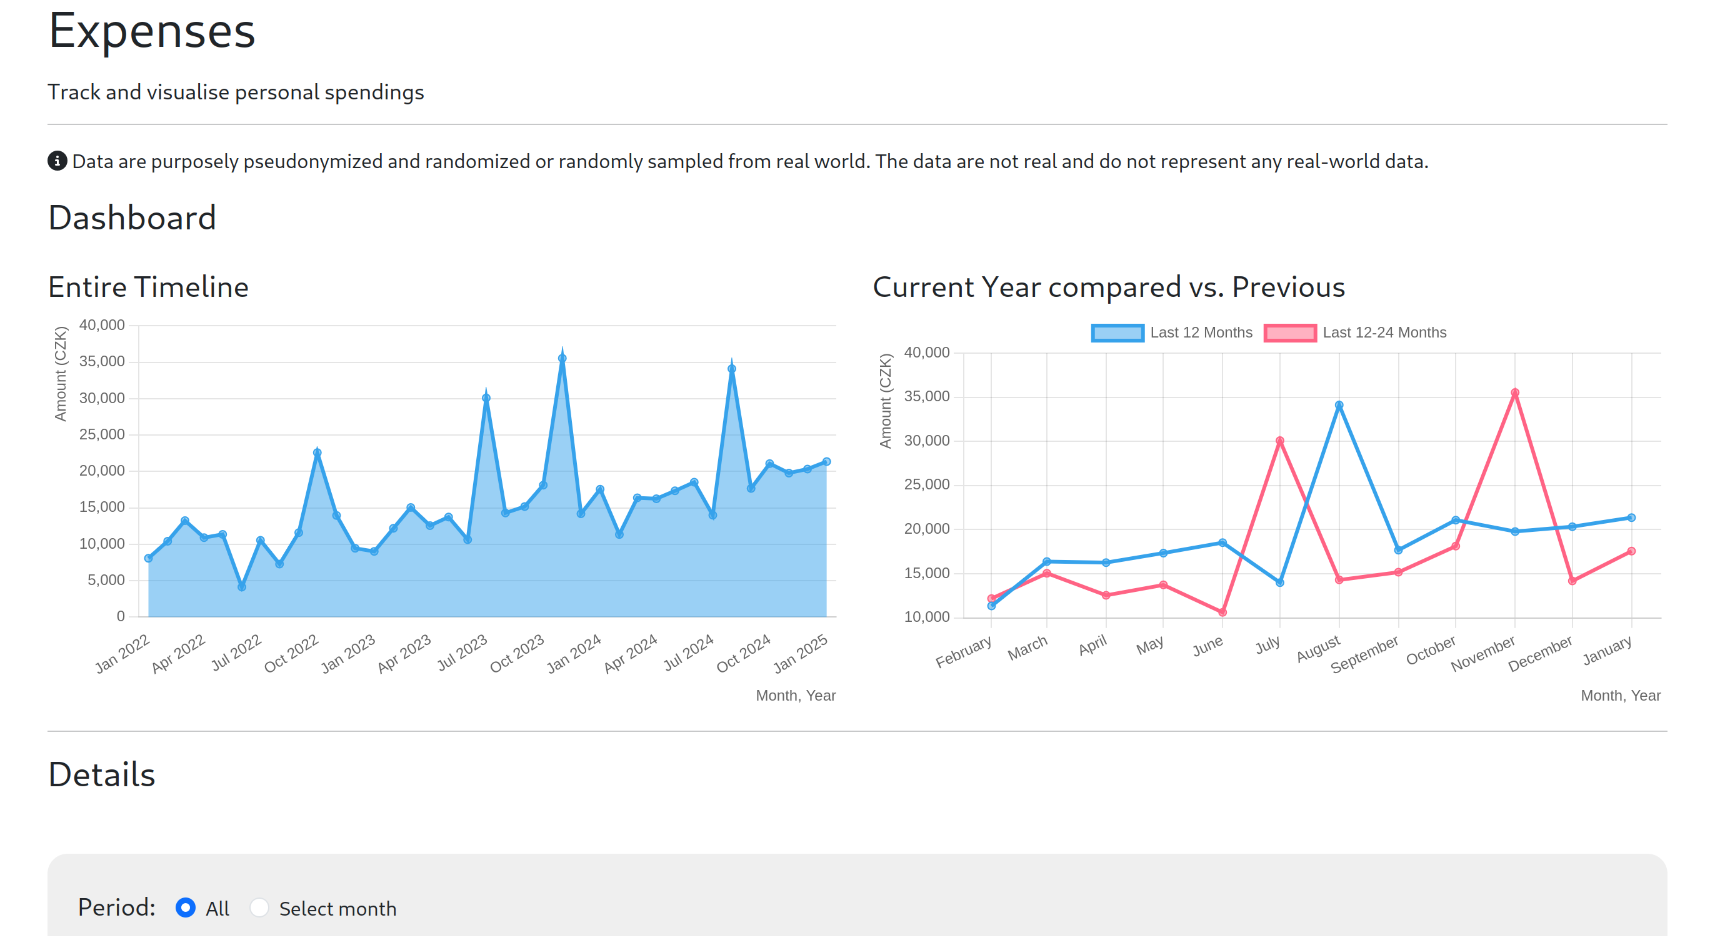
\includegraphics[width=0.8\textwidth]{image1.png}
            \caption{Entire Period}
        \end{figure}
        \begin{figure}
            \centering
            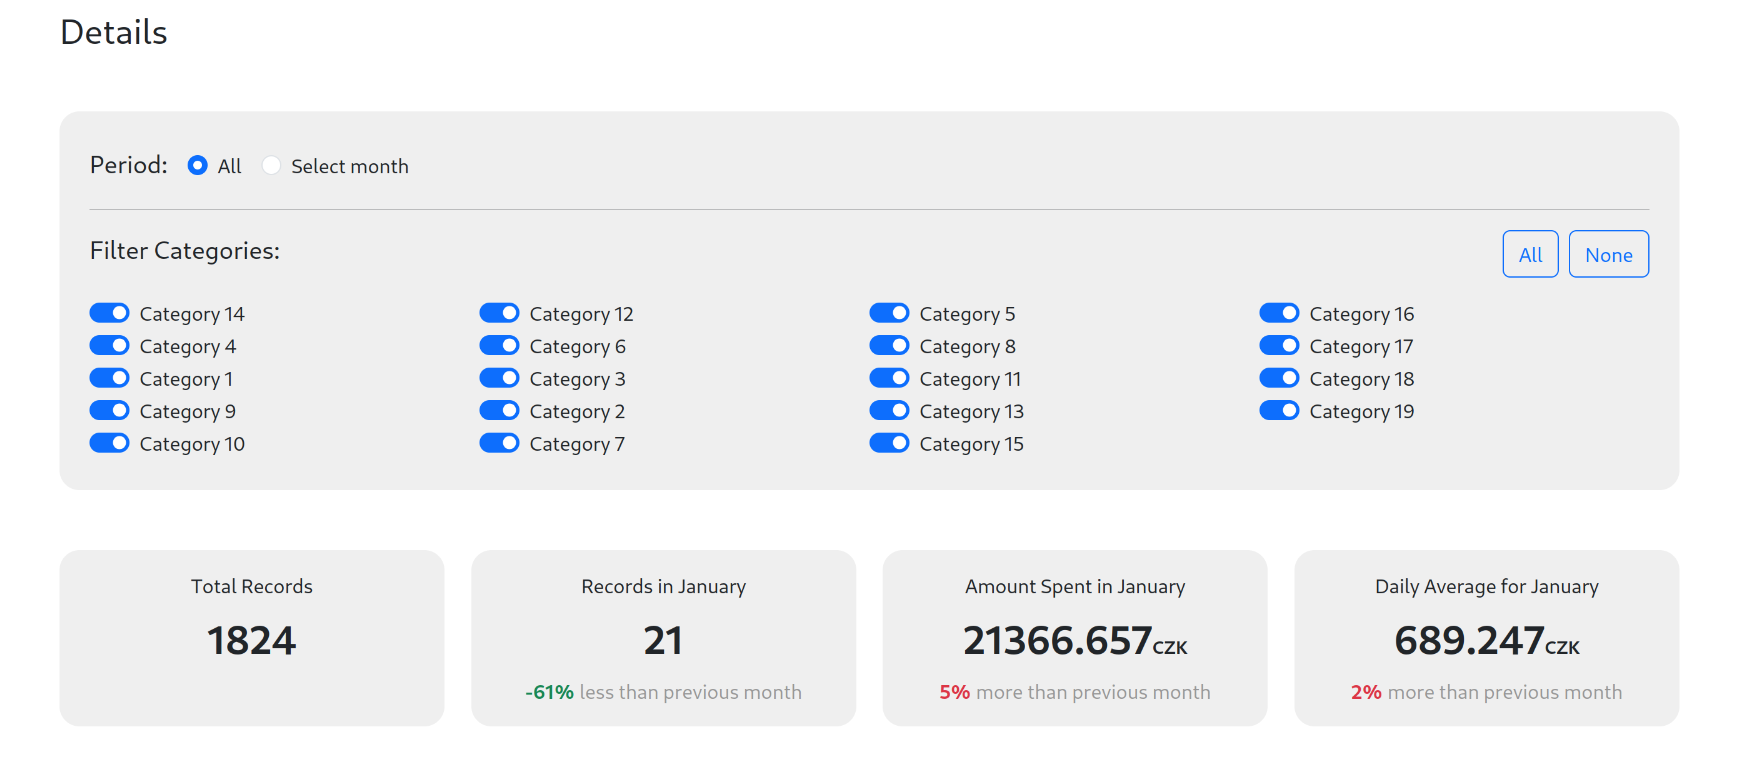
\includegraphics[width=0.8\textwidth]{image2.png}
            \caption{Filters}
        \end{figure}
        \begin{figure}
            \centering
            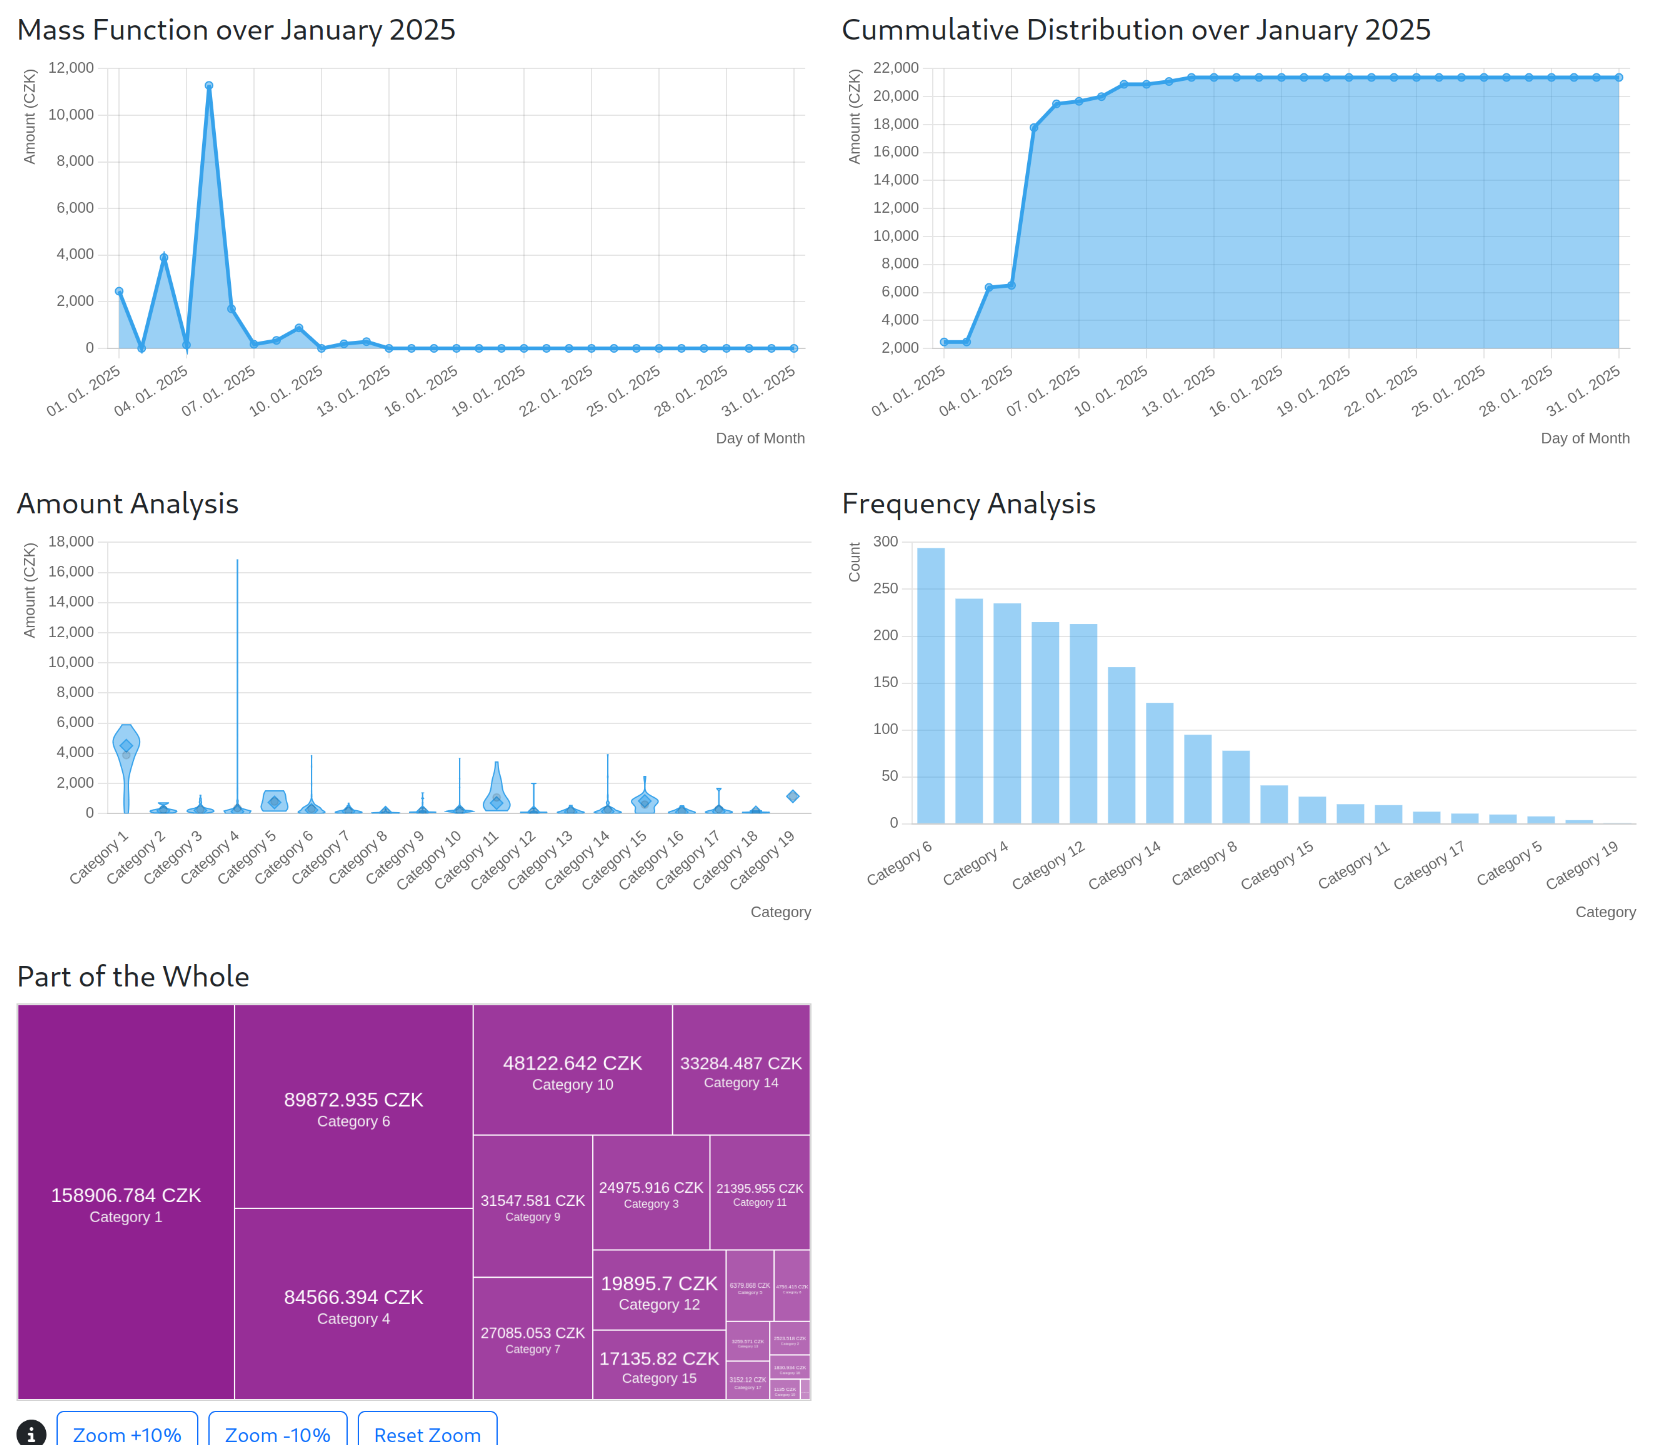
\includegraphics[width=0.8\textwidth]{image3.png}
            \caption{Additional Charts}
        \end{figure}
\end{document}
\makeatother
